\documentclass[]{article}
\usepackage[a4paper, margin=2.5cm]{geometry}
\usepackage{amsmath}
\usepackage{amsfonts}
\usepackage{amssymb}
\usepackage{mathtools}
\usepackage{amsthm}
\usepackage[many]{tcolorbox}
\usepackage{bm}
\usepackage{enumitem}

\newtheorem*{angabe*}{Angabe}
\newtheorem*{theorem*}{Satz}

\tcolorboxenvironment{angabe*}{
	colback=blue!5!white,
	boxrule=0pt,
	boxsep=1pt,
	left=2pt,right=2pt,top=2pt,bottom=2pt,
	oversize=2pt,
	sharp corners,
	before skip=\topsep,
	after skip=\topsep,
}

\tcolorboxenvironment{theorem*}{
	colback=red!5!white,
	boxrule=0pt,
	boxsep=1pt,
	left=2pt,right=2pt,top=2pt,bottom=2pt,
	oversize=2pt,
	sharp corners,
	before skip=\topsep,
	after skip=\topsep,
}

%opening
\title{Analysis 3 - Übung Nr. 10}
\author{Ida Hönigmann}

\begin{document}

\maketitle

\section{Sätze}

\begin{theorem*}[Integralsatz von Gauß]
	Ist $A$ ein offene und beschränkte Teilmenge des $\mathbb{R}^n$ mit $\mathcal{H}^{n-1}(\partial_sA)=0$, $\bm{f}:\bar{A}\rightarrow\mathbb{R}^n$ ein Vektorfeld aus $C(\bar{A})\cap C^1(A)$, so gilt wenn beide Integrale existieren
	\begin{align*}
		\int_A div\bm{f} d\lambda^n = \int_{\partial A} \bm{f}^\top \bm{n} d\mathcal{H}^{n-1}
	\end{align*}
	wobei $\nu$ den in das Äußere von $A$ zeigenden normierten Normalvektor auf $\partial A$ bezeichnet.
\end{theorem*}

\begin{theorem*}[Integralsatz von Stokes für die Ebene]
	Ist $A$ offen und beschränkt in $\mathbb{R}^2$ mit $\partial A \setminus \partial_r A$ endlich, sowie $\bm{f}:\bar{A}\rightarrow\mathbb{R}^2$ eine auf $\bar{A}$ stetige und auf $A$ stetig differenzierbare Funktion, so gilt:
	\begin{align*}
		\int_A rot\bm{f} d\lambda^2 = \int_{\partial A} \bm{f}\cdot \bm{t} ds,
	\end{align*}
	wobei $\bm{t}$ den normierten Tangentialvektor einer positiv orientierten Parametrisierung und $s$ die Weglänge bezeichnet.
\end{theorem*}

\begin{theorem*}[Integralsatz von Stokes im $\mathbb{R}^3$]
	Es sei $\Omega \subset \mathbb{R}^3$ das Bild einer beschränkten Teilmenge des $\mathbb{R}^2$ mit stückweise stetig differenzierbarem Rand unter einer $C^2$-Abbildung. Weiters sei $\bm{f}$ ein $C^1$-Vektorfeld auf einer offenen Obermenge von $\bar{\Omega}$. Dann gilt
	\begin{align*}
		\int_\Omega rot\bm{f}\cdot\bm{n}d\mathcal{H}^2 = \int_{\partial\Omega} \bm{f}^\top \cdot \bm{t} d\mathcal{H}^1,
	\end{align*}
	wobei $\bm{n}$ ein normiertes Normalvektorfeld auf $\Omega$ und $\bm{t}$ ein normiertes Tangentialvektorfeld an $\partial\Omega$ bezeichnet wobei die Orientierung von $\bm{n}$ und $\bm{t}$ so zu wählen ist, dass auf $\partial\Omega$ $\det(\bm{\nu}, \bm{t}, \bm{n}) > 0$ für ein in das Äußere von $\Omega$ zeigende Tangentialvektorfeld $\bm{\nu}$ auf $\partial\Omega$ gilt.
\end{theorem*}
\newpage

\section{Beispiele}

\subsection*{Beispiel 1}
\begin{angabe*}
	Sei $\bm{F}(x,y,z) := (xy, yz, x^2+y^2)^\top$. Betrachte den Zylindermantel
	\begin{align*}
		M := \{(x,y,z) \in \mathbb{R}^3: x^2+y^2=1, 0<z<1\}
	\end{align*}
	Berechnen Sie den Fluss des Vektorfeldes $\mathbf{F}$ durch die Fläche $M$:
	\begin{align*}
		\int_M \bm{F}^\top \cdot \bm{\nu} d\mathcal{H}^2
	\end{align*}
	wobei $\bm{\nu}$ den nach außen gerichteten normierten Normalvektor auf $M$ bezeichnet.
	Tun Sie das auf zwei Arten:
	\begin{enumerate}[label=(\roman*)]
		\item direkt
		\item mithilfe des Gauß'schen Integralsatzes.
	\end{enumerate}
\end{angabe*}

\begin{figure}[h!]
	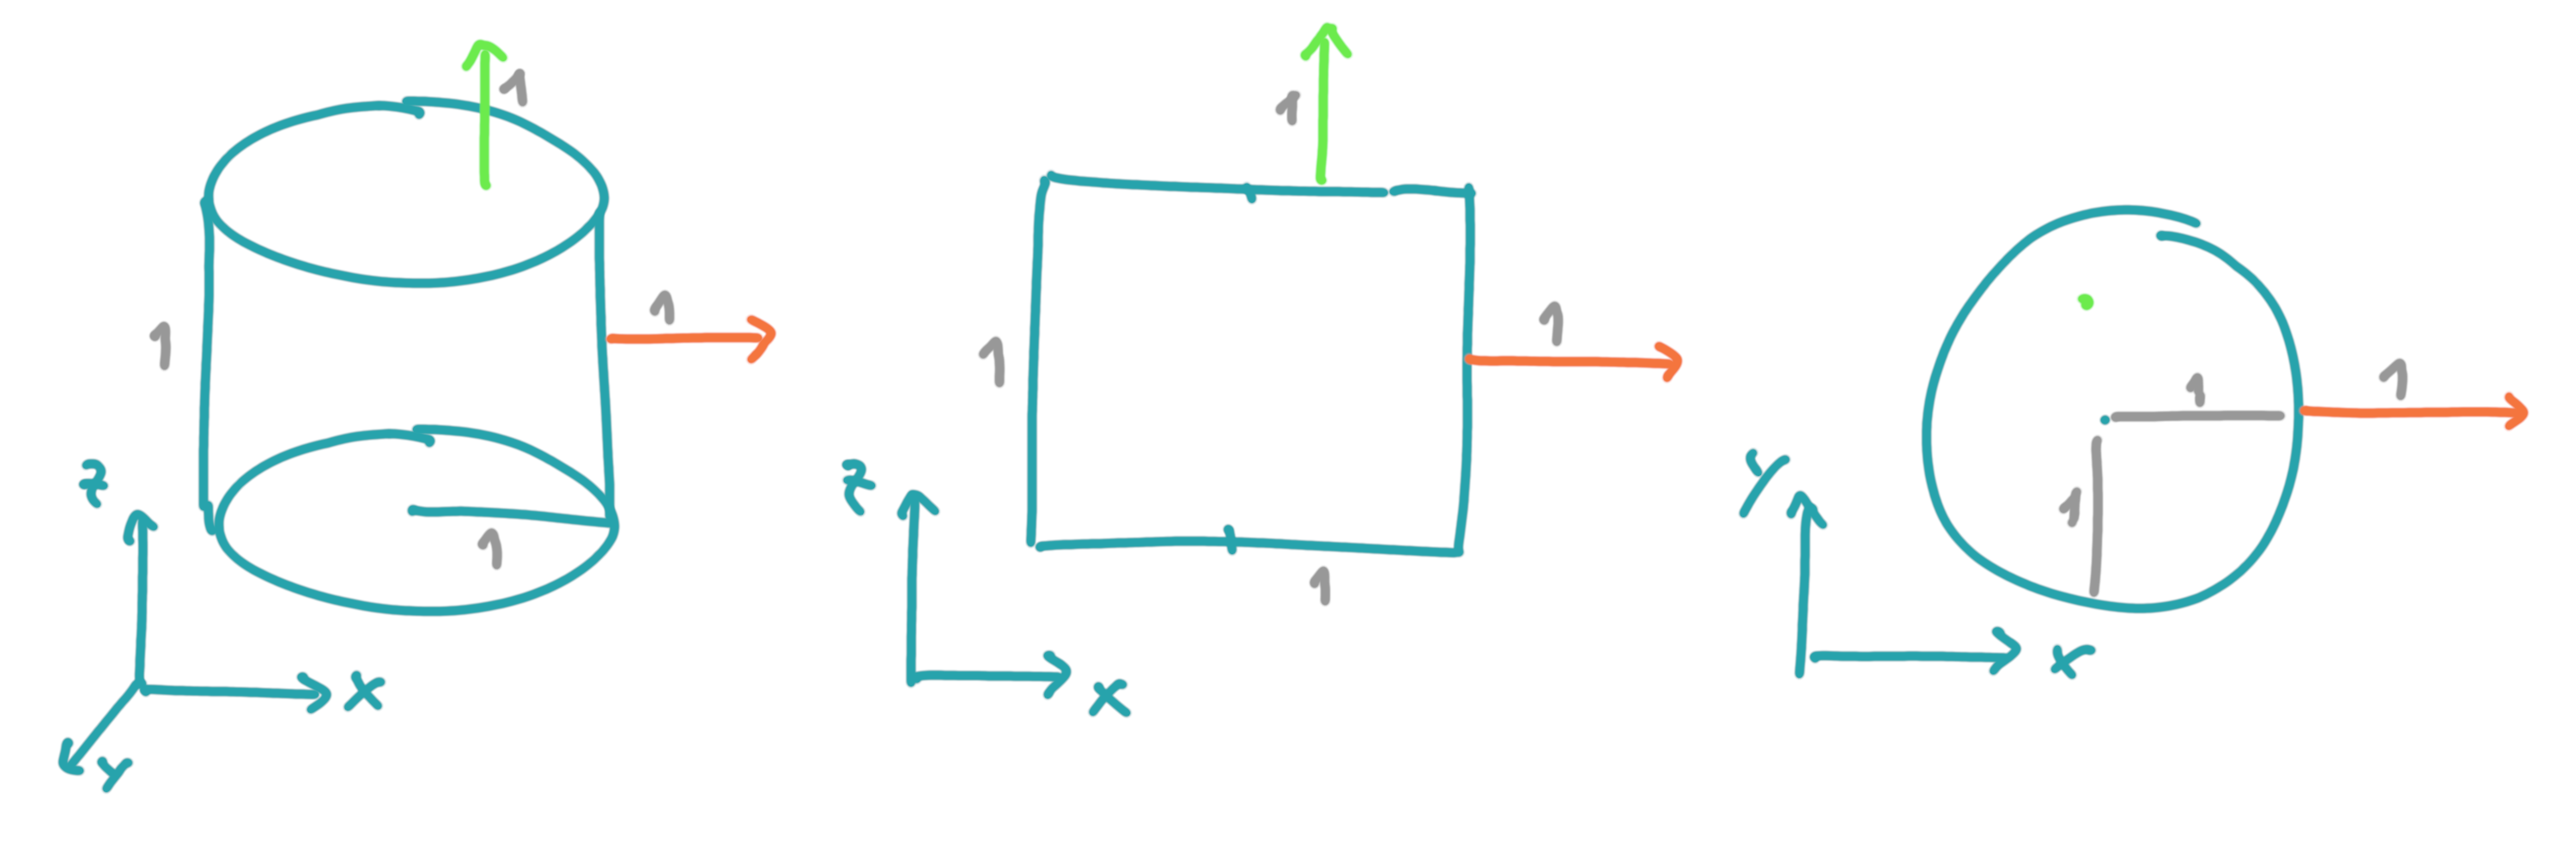
\includegraphics[width=\columnwidth]{bsp_1.png}
\end{figure}

\begin{enumerate}[label=(\roman*)]
	\item \textbf{direkt}:
	
	In jedem Punkt $(x,y,z) \in M$ gilt, dass der normierte Normalvektor
	\begin{align*}
		\bm{\nu} =
		\frac{1}{||\bm{\nu}||} \begin{pmatrix} \frac{\partial}{\partial x} x^2 + y^2 - 1\\ \frac{\partial}{\partial y} x^2 + y^2 - 1\\ \frac{\partial}{\partial z} x^2 + y^2 - 1 \end{pmatrix} =
		\frac{1}{\underbrace{\sqrt{4x^2 + 4y^2}}_{x^2+y^2=1} } \begin{pmatrix} 2x\\ 2y\\ 0 \end{pmatrix} = 
		\begin{pmatrix} x\\ y\\ 0 \end{pmatrix}.
	\end{align*}

	Es gilt also $\int_M \bm{F}^\top \bm{\nu} d\mathcal{H}^2 = \int_M x^2y + y^2z d\mathcal{H}^2$. Wir wollen nun zur Berechnung die Transformationsformel anwenden.
	\begin{align*}
		D := [0, 2\pi) \times (0,1) && \phi:D \rightarrow \mathbb{R}^2, (\theta, z) \mapsto (\cos(\theta), \sin(\theta), z)\\
		d\phi = \begin{pmatrix} -\sin(\theta) & 0 \\ \cos(\theta) & 0 \\ 0 & 1 \end{pmatrix} && \det(d\phi^\top d\phi) = \det\begin{pmatrix} \sin^2(\theta) + \cos^2(\theta) & 0 \\ 0 & 1 \end{pmatrix} = 1
	\end{align*}

	Offenbar gilt $\phi(D)=M$ und $\phi$ ist injektiv und eine $C^1$-Abbildung.

	\begin{align*}
		\int_M \bm{F}^\top \bm{\nu} d\mathcal{H}^2 = \int_{\phi(D)} x^2y + y^2z d\mathcal{H}^2 = \int_D \cos^2(\theta) \sin(\theta) + \sin^2(\theta) z d\lambda^2(\theta, z) =\\
		\int_{0}^{2\pi}\int_{0}^{1} \cos^2(\theta)\sin(\theta) dz d\theta + \int_{0}^{2\pi} \int_{0}^{1} \sin^2(\theta)z dz d\theta = \underbrace{\int_{0}^{2\pi} \cos^2(\theta) \sin(\theta) d\theta}_{=0} + \left.\frac{z^2}{2}\right\vert _0^1 \underbrace{\int_{0}^{2\pi} \sin^2(\theta) d\theta}_{=\pi} = \frac{\pi}{2}
	\end{align*}

	\item \textbf{mit Gauß'schem Integralsatz}:

	Wir betrachten zuerst $A:=\{(x,y,0)^\top\in \mathbb{R}^3: x^2+y^2 < 1\} = B_1^2(0)$ (der Boden des Zylinders) und $B:=\{(x,y,1)^\top \in \mathbb{R}^3: x^2+y^2 < 1\} = B_1^2(0)+(0,0,1)^\top$ (der Deckel des Zylinders). Offenbar gilt für $(x,y,0) \in A$, dass der Normalvektor $\bm{\nu} = (0,0,-1)^\top$ und für $(x,y,1) \in B$, dass $\bm{\nu} = (0,0,1)^\top$. Da $\bm{F}$ in der dritten Komponente nicht von $z$ abhängt gilt nun, dass sich die Summe der folgenden beiden Integrale aufhebt:
	\begin{align*}
		\int_A \bm{F}^\top \cdot \bm{\nu} d\mathcal{H}^2 + \int_B \bm{F}^\top \cdot \bm{\nu} d\mathcal{H}^2 = \int_{B_1^2(0)} -(x^2+y^2) d\mathcal{H}^2 + \int_{B_1^2(0)+(0,0,1)^\top} x^2+y^2 d\mathcal{H}^2 = \\
		-\int_{B_1^2(0)} x^2+y^2 d\mathcal{H}^2 + \int_{B_1^2(0)} x^2+y^2 d\mathcal{H}^2 = 0
	\end{align*}

	Damit erhalten wir, dass wenn wir mit $Z=\{(x,y,z)\in \mathbb{R}^3: x^2+y^2 < 1, 0<z<1\}$ den Zylinder bezeichnen, gilt
	\begin{align*}
		\int_{\partial Z} \bm{F}^\top \cdot \bm{\nu} d\mathcal{H}^2 = \int_M \bm{F}^\top \cdot \bm{\nu} d\mathcal{H}^2
	\end{align*}

	Um den Integralsatz von Gauß anwenden zu können müssen wir überprüfen ob
	\begin{itemize}
		\item $Z$ eine offene, beschränkte Teilmenge des $\mathbb{R}^3$ ist; was klarerweise gilt
		\item $\mathcal{H}^2(\partial_sZ)=0$ was gilt da $\partial_sZ = \{(x,y,0): x^2+y^2=1\} \cup \{(x,y,1): x^2+y^2=1\}$ und beide diese Mengen haben endliches eindimensionales Hausdorffmaß (genauer $\mathcal{H}^1(\text{Kreisrand})=2\pi$) und somit zweidimensionales Hausdorffmaß Null haben müssen ($\mathcal{H}^2(\text{Kreisrand})=0$).
		\item $\bm{F}:\bar{Z} \rightarrow \mathbb{R}^3 \in C(\bar{Z}) \cap C^1(Z)$, da $\bm{F}$ offenbar stetig ist und
		\begin{align*}
			D\bm{F} = \begin{pmatrix}
				y & x & 0\\ 0 & z & y\\ 2x & 2y & 0
			\end{pmatrix}
		\end{align*}
		ist stetig.
	\end{itemize}
	
	Also gilt nun
	\begin{align*}
		\int_{\partial_Z} \bm{F}^\top \cdot \nu d\mathcal{H}^2 = \int_Z div\bm{F} d\lambda^3 = \int_Z \frac{\partial F_1}{\partial x} + \frac{\partial F_2}{\partial y} + \frac{\partial F_3}{\partial z} d\lambda^3 = \int_Z y + z d\lambda^3
	\end{align*}

	Zur Berechnung verwenden wir wieder den Transformationssatz
	\begin{align*}
		D := (0,1)\times[0,2\pi)\times(0,1) && \phi:D\rightarrow\mathbb{R}^3, (r,\theta,z) \mapsto (r\cos(\theta), r\sin(\theta), z)^\top && \det(d\phi^T d\phi) = r^2
	\end{align*}

	wobei $D$ ist eine offene Teilmenge des $\mathbb{R}^3$, $\phi$ ist eine injektive $C^1$-Abbildung und $Z=\phi(D)$. Damit folgt 
	\begin{align*}
		\int_{\phi(D)} y + z d\lambda^3 = \int_D (r\sin(\theta) + z)r d\lambda^3 = \int_{0}^{1} \int_{0}^{2\pi} \int_{0}^{1} r^2 \sin(\theta) dz d\theta dr + \int_{0}^{1} \int_{0}^{2\pi} \int_{0}^{1} rz dz d\theta dr = \\
		\int_{0}^{1} r^2 \left.(-\cos(\theta))\right\vert_0^{2\pi} dr + 2\pi \int_{0}^{1} r \left. \frac{z^2}{2}\right\vert_0^1 dr = 0 + 2\pi \int_0^1 \frac{1}{2} r dr = \pi \left. \frac{r^2}{2}\right\vert_0^1 = \frac{\pi}{2}.
	\end{align*}

\end{enumerate}
\newpage

\subsection*{Beispiel 2}
\begin{angabe*}
	Sei $\bm{F}(x,y,z):=(xz, xy, z^2-x)^\top$. Betrachte das Gebiet
	\begin{align*}
		\Omega := \{(x,y,z)\in \mathbb{R}^3: 0<x<1, 0<y<x+1, 0<z<x+y\}.
	\end{align*}
	Berechnen Sie den Fluss des Vektorfeldes $\bm{F}$ durch den Rand von $\Omega$.
\end{angabe*}

\begin{figure}[h!]
	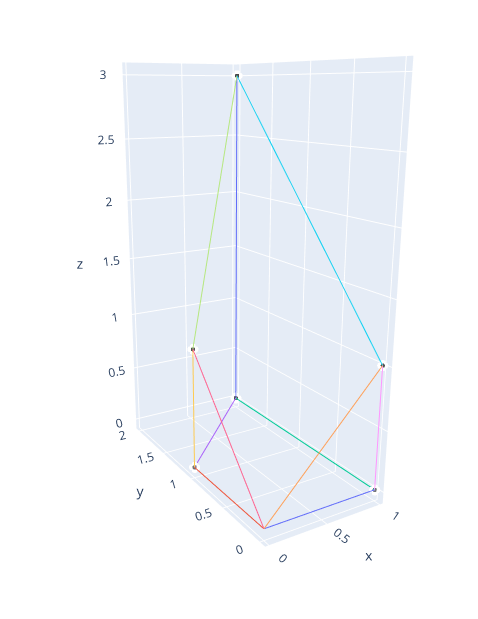
\includegraphics[width=0.5\columnwidth]{bsp_2.png}
\end{figure}

Gesucht ist
\begin{align*}
	\int_{\partial \Omega} \bm{F}^\top \cdot \bm{\nu} d\mathcal{H}^2
\end{align*}
weshalb wir den Gauß'schen Integralsatz verwenden wollen. Daher prüfen wir zuerst die Bedingungen:
\begin{itemize}
	\item $\Omega$ ist offen und beschränkt: offen ist aus der Definition klar, Beschränktheit folgt aus $\Omega \subseteq (0,1)\times(0,2)\times(0,3)$.
	\item $\mathcal{H}^2(\partial_s\Omega) = 0$, da $\partial_s\Omega$ aus 11 Kanten (und 7 Ecken) besteht (siehe Grafik) und diese alle endliches eindimensionales Hausdorffmaß besitzen und daher $\mathcal{H}^2(\partial_s\Omega) = 0$.
	\item $\bm{F}:\overline{\Omega} \rightarrow \mathbb{R}^3 \in C(\overline{\Omega}) \cap C^1(\Omega)$, da $\bm{F}$ offenbar stetig ist und
	\begin{align*}
		D\bm{F} = \begin{pmatrix}
			z & 0 & x\\ y & x & 0\\ 2x & -2y & 0\\
		\end{pmatrix}
	\end{align*}
	ist stetig.
\end{itemize}

Gemeinsam mit $div\bm{F} = \sum_{i=1}^{3} \partial f_i / \partial x_i = x+z$ und dem Gauß'schen Integralsatz ergibt sich
\begin{align*}
	\int_{\partial\Omega} \bm{F}^\top \bm{\nu} d\mathcal{H}^2 = \int_\Omega div\bm{F} d\lambda^3 = \int_0^1 \int_0^{x+1} \int_0^{x+y} x+z dzdydx\\
	\int_0^1 \int_0^{x+1} \int_0^{x+y} x dzdydx = \int_0^1 x \int_0^{x+1} x+y dy dx = \int_0^1 x\left(x(x+1) + \left.\frac{y^2}{2}\right\vert_0^{x+1}\right) dx =\\
	\int_0^1 x \left(x^2+x + \frac{(x+1)^2}{2}\right) dx = \int_0^1 x^3 + x^2 + \frac{x}{2} (x^2+2x+1) dx = \int_0^1 \frac{3}{2} x^3 + 2 x^2 + \frac{1}{2} x dx = \frac{31}{24}\\
	\int_0^1 \int_0^{x+1} \int_0^{x+y} z dzdydx = \int_0^1 \int_0^{x+1} \frac{(x+y)^2}{2} dy dx = \frac{1}{2} \int_0^1 \int_x^{2x+1} u^2 du dx = \frac{1}{2} \int_0^1 \left.\frac{u^3}{3}\right\vert_x^{2x+1} dx =\\
	\frac{1}{6} \int_0^1 (2x+1)^3 - x^3 dx = \frac{1}{6} \left(\int_1^3 \frac{v^3}{2} dv - \left. \frac{x^4}{4}\right\vert_0^1\right) = \frac{1}{6} \left(\frac{1}{2} \left.\frac{v^3}{4}\right\vert_1^3 - \frac{1}{4}\right) = \frac{13}{8}\\
	\implies \int_{\partial\Omega} \bm{F}^\top \bm{\nu} d\mathcal{H}^2 = \frac{31}{24} + \frac{13}{8} = \frac{35}{12}
\end{align*}
\newpage

\subsection*{Beispiel 3}
\begin{angabe*}
	Verifizieren Sie den Gauß'schen Integralsatz für das Gebiet
	\begin{align*}
		\Omega := \{(x,y,z) \in \mathbb{R}^3: 0<z<1-x^2-y^2\}
	\end{align*}
	und das Vektorfeld
	\begin{align*}
		\bm{F}(x,y,z) := (x, x+y, x^2+z)^\top,
	\end{align*}
	d.h., berechnen Sie die beiden Integrale und überprüfen Sie deren Gleichheit.
\end{angabe*}

\begin{figure}[h!]
	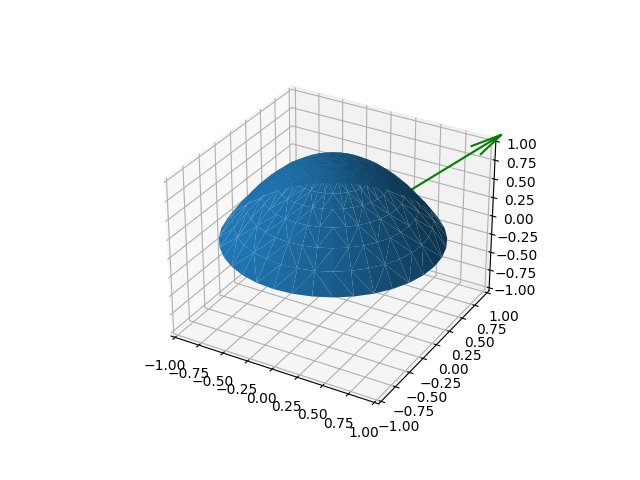
\includegraphics[width=0.5\columnwidth]{bsp_3.png}
\end{figure}

Zuerst berechnen wir $\int_\Omega div\bm{F} d\lambda^3$:
\begin{align*}
	div\bm{F} = \frac{\partial f_1}{\partial x} + \frac{\partial f_2}{\partial y} + \frac{\partial f_3}{\partial z} = 1 + 1 + 1 = 3 && \implies	\int_\Omega div\bm{F} d\lambda^3 = 3 \int_\Omega d\lambda^3
\end{align*}

Mit der Transformationsformel für $D:=\{(r,\theta, z): r \in (0,1), \theta \in [0,2\pi), z \in (0,1-r^2)\}$ und $\phi(r,\theta, z) = (r\cos(\theta), r\sin(\theta), z)$ gilt $\det(d\phi^\top d\phi) = r^2$ sowie $\Omega=\phi(D)$ und es folgt
\begin{align*}
	3 \int_\Omega d\lambda^3 = 3 \int_{0}^{1} \int_{0}^{2\pi} \int_{0}^{1-r^2} r dz d\theta dr = 6\pi \int_{0}^{1} r(1-r^2) dr = 6\pi \left(\int_{0}^{1} r dr - \int_{0}^{1} r^3 dr\right) = 6\pi (\frac{1}{2}-\frac{1}{4}) = \frac{3\pi}{2}
\end{align*}

Für die Berechnung von $\int_{\partial\Omega} \bm{F}^\top \bm{\nu} d\mathcal{H}^2$ müssen wir uns zuerst überlegen wie der normierte Normalvektor auf $\partial\Omega$ aussieht.
\begin{align*}
	\partial\Omega = A_1 \cup A_2 = \{(x,y,0)\in\mathbb{R}^3: x^2+y^2 < 1\} \cup \{(x,y,1-x^2-y^2)\}\in\mathbb{R}^3: x^2+y^2 < 1\}\\
	\text{Auf } A_1: \bm{\nu} = (0,0,-1)^\top\\
	\text{Auf } A_2: \tilde{\bm{\nu}} = \left(-\frac{\partial}{\partial x} (1-x^2-y^2),-\frac{\partial}{\partial y} (1-x^2-y^2), 1\right)^\top = (2x, 2y, 1)^\top\\
	||\tilde{\bm{\nu}}|| = \sqrt{4x^2+4y^2+1} \implies \bm{\nu} = \frac{\tilde{\bm{\nu}}}{||\tilde{\bm{\nu}}||}
\end{align*}

Nun gilt
\begin{align*}
	\int_{\partial\Omega} \bm{F}^\top \bm{\nu} d\mathcal{H}^2 = \int_{A_1} \bm{F}^\top \bm{\nu} d\mathcal{H}^2 + \int_{A_2} \bm{F}^\top \bm{\nu} d\mathcal{H}^2\\
	\int_{A_1} \bm{F}^\top \bm{\nu} d\mathcal{H}^2 = \int_{A_1} (x, x+y, x^2)\cdot \begin{pmatrix}0\\ 0\\ -1\end{pmatrix} d\mathcal{H}^2 = \int_{A_1} -x^2 d\mathcal{H}^2\\
	\int_{A_2} \bm{F}^\top \bm{\nu} d\mathcal{H}^2 = \int_{A_2} \frac{1}{\sqrt{4(x^2+y^2)+1}} (x, x+y, 1-y^2)\cdot \begin{pmatrix}2x\\ 2y\\ 1\end{pmatrix} d\mathcal{H}^2 =\\
	\int_{A_2} \frac{2x^2 + 2xy + 2y^2 + 1 - y^2}{\sqrt{4(x^2+y^2)+1}} d\mathcal{H}^2 = \int_{A_2} \frac{2x^2 + 2xy + y^2 + 1}{\sqrt{4(x^2+y^2)+1}} d\mathcal{H}^2
\end{align*}

Für die Transformationsformel sein nun $D:=(0,1)\times[0,2\pi)$, $\phi_1(r, \theta)=(r\cos(\theta), r\sin(\theta), 0)$ und $\phi_2(r, \theta)=(r\cos(\theta), r\sin(\theta), 1-r^2)$, dann gilt $A_1=\phi_1(D)$ und $A_2=\phi_2(D)$, sowie $\det(d\phi_1^\top d\phi_1) = r^2$ und $\det(d\phi_2^\top d\phi_2) = r^2(4r^2+1)$.

\begin{align*}
	\int_{A_1} -x^2 d\mathcal{H}^2 = \int_{0}^{1} \int_{0}^{2\pi} -r^2 \cos^2(\theta) r d\theta dr = -\int_{0}^{1} r^3 \int_{0}^{2\pi} \cos^2(\theta) d\theta dr = -\pi \int_{0}^{1} r^3 dr = -\frac{\pi}{4}\\
	\int_{A_2} \frac{2x^2 + 2xy + y^2 + 1}{\sqrt{4(x^2+y^2)+1}} d\mathcal{H}^2 = \int_{0}^{1}\int_{0}^{2\pi} \frac{2r^2\cos^2(\theta)+2r^2\cos(\theta)\sin(\theta)+r^2\sin^2(\theta)+1}{\sqrt{4r^2 + 1}} r\sqrt{4r^2+1} d\theta dr =\\
	\int_{0}^{1} 2r^3 \int_{0}^{2\pi} \cos^2(\theta) d\theta + 2r^3 \int_{0}^{2\pi} \cos(\theta)\sin(\theta) d\theta + r^3 \int_{0}^{2\pi} \sin^2(\theta) d\theta + r \int_{0}^{2\pi} d\theta dr =\\
	\int_{0}^{1} 2\pi r^3 + \pi r^3 + 2\pi r dr = \frac{2\pi}{4} + \frac{\pi}{4} + \frac{2\pi}{2} = \frac{7\pi}{4}\\
	\implies \int_{\partial\Omega} \bm{F}^\top \bm{\nu} d\mathcal{H}^2 = -\frac{\pi}{4} + \frac{7\pi}{4} = \frac{3\pi}{2}
\end{align*}
\newpage

\subsection*{Beispiel 4}
\begin{angabe*}
	Sei $A \subseteq \mathbb{R}^3$ offen. Sei $f\in C^2(A)$ eine reelle Funktion, sei $\bm{F} \in C^2(A;\mathbb{R}^3)$ ein Vektorfeld. Zeigen Sie
	\begin{enumerate}[label=(\roman*)]
		\item $rot\nabla f = \bm{0}$,
		\item $div rot \bm{F} = 0$
	\end{enumerate}
\end{angabe*}

\begin{enumerate}[label=(\roman*)]
	\item Da die Reihenfolge bei Differenzieren von $f$ egal ist ergibt sich
	\begin{align*}
		\nabla f = \begin{pmatrix}
			\frac{\partial f}{\partial x} \\ \frac{\partial f}{\partial x} \\ \frac{\partial f}{\partial x}
		\end{pmatrix} =: (f_1, f_2, f_3)^\top &&
		rot \nabla f = \begin{pmatrix}
			\frac{\partial f_3}{\partial y} - \frac{\partial f_2}{\partial z}\\
			\frac{\partial f_1}{\partial z} - \frac{\partial f_3}{\partial x}\\
			\frac{\partial f_2}{\partial x} - \frac{\partial f_1}{\partial y}\\
		\end{pmatrix} = \begin{pmatrix} 
		\frac{\partial^2 f}{\partial y \partial z} - \frac{\partial^2 f}{\partial z \partial y}\\
		\frac{\partial^2 f}{\partial z \partial x} - \frac{\partial^2 f}{\partial x \partial z}\\
		\frac{\partial^2 f}{\partial x \partial y} - \frac{\partial^2 f}{\partial y \partial x}\\
		\end{pmatrix} = \begin{pmatrix}
			0 \\ 0 \\ 0
		\end{pmatrix}
	\end{align*}

	\item Sei $\bm{F} = (f_1, f_2, f_3)$, dann gilt
	\begin{align*}
		rot \bm{F} = \begin{pmatrix}
			\frac{\partial f_3}{\partial y} - \frac{\partial f_2}{\partial z}\\
			\frac{\partial f_1}{\partial z} - \frac{\partial f_3}{\partial x}\\
			\frac{\partial f_2}{\partial x} - \frac{\partial f_1}{\partial y}\\
		\end{pmatrix}\\
		\text{div rot} \bm{F} = \frac{\partial}{\partial x} \left(\frac{\partial f_3}{\partial y} - \frac{\partial f_2}{\partial z}\right) + \frac{\partial}{\partial y} \left(\frac{\partial f_1}{\partial z} - \frac{\partial f_3}{\partial x}\right) + \frac{\partial}{\partial z} \left(\frac{\partial f_2}{\partial x} - \frac{\partial f_1}{\partial y}\right) = \\
		\frac{\partial^2 f_3}{\partial x \partial y} - \frac{\partial^2 f_2}{\partial x \partial z} + \frac{\partial^2 f_1}{\partial y \partial z} - \frac{\partial^2 f_3}{\partial x \partial y} + \frac{\partial^2 f_2}{\partial x \partial z} - \frac{\partial^2 f_1}{\partial y \partial z} = 0
	\end{align*}
\end{enumerate}
\newpage

\subsection*{Beispiel 5}
\begin{angabe*}
	Sei $B \subseteq \mathbb{R}^2$ die offene Einheitskreisscheibe in $\mathbb{R}^2$. Wir schreiben das Wegintegral
	\begin{align*}
		\int_\gamma \begin{pmatrix}	f_1(\bm{x})\\ f_2(\bm{x}) \end{pmatrix} d\bm{x} =: \int_\gamma f_1(\bm{x}) dx + f_2(\bm{x}) dy.
	\end{align*}
	Berechnen Sie das Wegintegral
	\begin{align*}
		\int_{\partial B} (x-y^3) dx + y^3 dy
	\end{align*}
	\begin{enumerate}[label*=(\roman*)]
		\item direkt
		\item mithilfe des Stoke'schen Integralsatzes.
	\end{enumerate}
\end{angabe*}

\begin{enumerate}[label*=(\roman*)]
	\item \textbf{direkt}:
	
	Wir setzen $D:=[0,2\pi)$ und $\phi(\theta):=(\cos(\theta), \sin(\theta))$, dann wird der Weg des Wegintegrals wird durch $\phi(D)$ beschrieben. Wegen $\int_\gamma f(x) dx = \int_{[a, b]} f(\gamma(t)) \gamma'(t) dt$ gilt:
	
	\begin{align*}
		\int_{\partial B} \begin{pmatrix} x-y^3\\ y^3 \end{pmatrix} d(x,y) = \int_{0}^{2\pi} \begin{pmatrix} \cos(\theta)-\sin^3(\theta)\\ \sin^3(\theta) \end{pmatrix} \begin{pmatrix} \cos(\theta)\\ \sin(\theta) \end{pmatrix}' d\theta =\\
		\int_{0}^{2\pi} -\sin(\theta)\cos(\theta) + \sin^4(\theta) + \sin^3(\theta)\cos(\theta) d\theta = 0 + \frac{3\pi}{4} + 0 = \frac{3\pi}{4}
	\end{align*}

	\item \textbf{mithilfe des Stoke'schen Integralsatzes}:
	
	Auf der Einheitskreisscheibe ist offenbar für jeden Punkt $(x,y)^\top$ der Vektor $(x,y)^\top$ ein normierter Normalvektor, daher sind die beiden Tangentialvektor an der Stelle $(-y, x)^\top$ und $(y, -x)^\top$, wobei der erste der positiven Orientierung entspricht.
	
	Zuerst prüfen wir die Vorraussetzungen für den Integralsatz von Stokes für die Ebene:
	\begin{itemize}
		\item $B$ ist klarerweise offen und beschränkt in $\mathbb{R}^2$
		\item $\partial B \setminus \partial_r B = \emptyset$ also endlich
		\item $f:\bar{B}\rightarrow\mathbb{R}^2 \in C(\bar{B}) \cap C^1(B)$: stetig auf $\bar{B}$ ist klar;
		\begin{align*}
			Df = \begin{pmatrix} 1 & -3y^2\\ 0 & 3y^2 \end{pmatrix}
		\end{align*}
		ist stetig auf $B$.
	\end{itemize}

	Daher gilt nun
	\begin{align*}
		\int_{0}^{2\pi} \begin{pmatrix} \cos(\theta)-\sin^3(\theta)\\ \sin^3(\theta) \end{pmatrix} \begin{pmatrix} -\sin(\theta)\\ \cos(\theta) \end{pmatrix} d\theta = \int_{\partial B} \bm{f} \cdot \bm{t} ds = \int_B rot\bm{f} d\lambda^2 = \\
		\int_B \frac{\partial f_2}{\partial x} - \frac{\partial f_1}{\partial y} d\lambda^2 =		\int_B 0 - (-3y^2) d\lambda^2 = 3 \int_B y^2 d\lambda^2
	\end{align*}

	Mit der Transformationssformel für $D:=(0,1)\times[0,2\pi)$ und $\phi(r,\theta):=(r\cos(\theta), r\sin(\theta))^\top$ gilt $\det(d\phi^\top d\phi) = r^2$ und es folgt:
	\begin{align*}
		3 \int_B y^2 d\lambda^2 = 3 \int_{0}^{1} \int_{0}^{2\pi} r^2 \sin^2(\theta) r d\theta dr = 3\pi \int_{0}^{1} r^3 dr = \frac{3\pi}{4}
	\end{align*}
\end{enumerate}
\newpage

\subsection*{Beispiel 6}
\begin{angabe*}
	Sei $\bm{F}(x,y,z):=(1-xy, xz, x+z)^\top$. Betrachte das hyperbolische Paraboloid
	\begin{align*}
		\Omega := \{(x,y,z) \in \mathbb{R}^3: z = x^2-y^2, x^2+y^2 < 1\}.
	\end{align*}
	Verifizieren Sie den Stoke'schen Integralsatz für $\bm{F}$ auf $\Omega$.
\end{angabe*}

\begin{figure}[h!]
	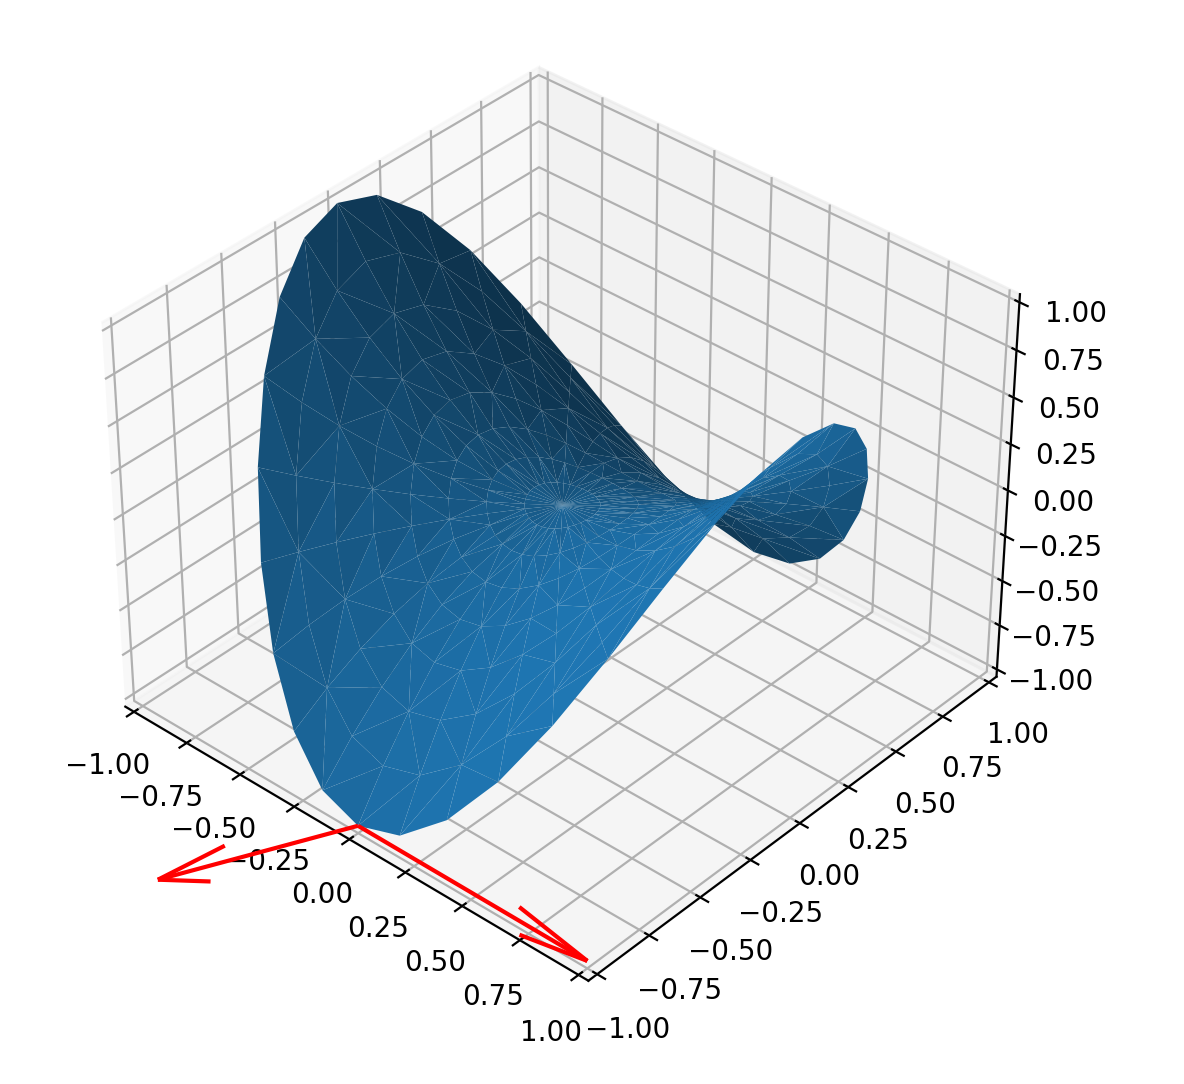
\includegraphics[width=0.5\columnwidth]{bsp_6.png}
\end{figure}

Zuerst wollen wir die benötigten Normal- und Tangentialvektoren berechnen.
Sei $(x,y,z) \in \Omega$, dann ist
\begin{align*}
	\tilde{n} := (-\frac{\partial x^2-y^2}{\partial x}, -\frac{\partial x^2-y^2}{\partial y}, 1)^\top = (-2x, 2y, 1)^\top
\end{align*}
ein Normalvektor auf $\Omega$ im Punkt $(x,y,z)$. Normieren ergibt
\begin{align*}
	n:= \frac{\tilde{n}}{||\tilde{n}||} = \frac{1}{\sqrt{4(x^2+y^2)+1}}(-2x, 2y, 1)^\top
\end{align*}

Sei nun $(x,y,z) \in \partial \Omega$ also aus dem Rand $\partial\Omega = \{(x,y,z) \in \mathbb{R}^3: z=x^2-y^2, x^2+y^2=1\}$. Dann ist die Polarkoordinatendarstellung gleich $(\cos(\theta), \sin(\theta), \cos^2(\theta) - \sin^2(\theta))$ und ein Tangentialvektor an dem Punkt gleich
\begin{align*}
	\tilde{\bm{t}} = \left(\frac{\partial}{\partial \theta} \cos(\theta), \frac{\partial}{\partial \theta} \sin(\theta), \frac{\partial}{\partial \theta} \cos^2(\theta)-\sin^2(\theta)\right)^\top = (-\sin(\theta), \cos(\theta), -4\sin(\theta)\cos(\theta))^\top = (-y, x, -4xy)^\top\\
\end{align*}
\begin{align*}
	||\tilde{\bm{t}}|| = \sqrt{x^2+y^2+16x^2*y^2} = \sqrt{16x^2y^2+1} && \bm{t} := \frac{\tilde{\bm{t}}}{||\tilde{\bm{t}}||}
\end{align*}

Nun berechnen wir $\int_\Omega rot\bm{f} \cdot \bm{n} d\mathcal{H}^2$:
\begin{align*}
	rot \bm{f} = \left(\frac{\partial f_3}{\partial y} - \frac{\partial f_2}{\partial z},
					   \frac{\partial f_1}{\partial z} - \frac{\partial f_3}{\partial x},
					   \frac{\partial f_2}{\partial x} - \frac{\partial f_1}{\partial y}\right)^\top =
	(0-x, 0-1, z-(-x))^\top = (-x, -1, x+z)^\top\\
	\int_\Omega rot\bm{f} \cdot \bm{n} d\mathcal{H}^2 = \int_\Omega \frac{1}{\sqrt{4(x^2+y^2)+1}} (-x, -1, x+z) \cdot \begin{pmatrix} -2x\\ 2y\\ 1 \end{pmatrix} d\mathcal{H}^2 =\\
	\int_\Omega \frac{2x^2 - 2y + x + z}{\sqrt{4(x^2+y^2)+1}} d\mathcal{H}^2 = \int_\Omega \frac{3x^2 - y^2 + x - 2y}{\sqrt{4(x^2+y^2)+1}} d\mathcal{H}^2
\end{align*}

Die Transformationsformel für $D:=(0,1)\times[0,2\pi)$ und $\phi(r, \theta) = (r\cos(\theta), r\sin(\theta))$ liefert uns $\det(d\phi^\top d\phi) = r^2$ und
\begin{align*}
	\int_\Omega \frac{3x^2 - y^2 + x - 2y}{\sqrt{4(x^2+y^2)+1}} d\mathcal{H}^2 = \int_{0}^{1} \int_{0}^{2\pi} \frac{3r^2\cos^2(\theta) - r^2\sin^2(\theta) + r\cos(\theta) - 2r\sin(\theta)}{\sqrt{4(r^2\cos^2(\theta)+r^2\sin^2(\theta))+1}} r d\theta dr =\\
	\int_{0}^{1} \frac{r}{\sqrt{4r^2 + 1}} \left(3r^2\int_{0}^{2\pi} \cos^2(\theta) d\theta - r^2\int_{0}^{2\pi} \sin^2(\theta) d\theta + r\int_{0}^{2\pi} \cos(\theta) d\theta - 2r\int_{0}^{2\pi} \sin(\theta) d\theta \right) dr = \\
	\int_{0}^{1} \frac{r}{\sqrt{4r^2 + 1}} (3\pi r^2 - \pi r^2) dr = 2\pi \int_{0}^{1} \frac{r^3}{\sqrt{4r^2+1}} dr = 2\pi \left. \frac{1}{24} (2r^2-1)\sqrt{4r^2 + 1}\right\vert_0^1 =  \frac{\pi}{12} (\sqrt{5} + 1)
\end{align*}

Nun zur Berechnung von $\int_{\partial\Omega} \bm{F}^\top \cdot \bm{t} d\mathcal{H}^1$:
\begin{align*}
	\int_{\partial\Omega} \bm{F}^\top \cdot \bm{t} d\mathcal{H}^1 = \int_{\partial\Omega} \frac{-y + xy^2 + x^2z - 4x^2y - 4xyz}{\sqrt{16x^2y^2+1}} d\mathcal{H}^1 =\\
	\int_{\partial\Omega} \frac{-y+xy^2+x^4-x^2y^2-8x^2y+4y^3}{\sqrt{16x^2y^2+1}} d\mathcal{H}^1 = \int_0^{2\pi} \frac{num}{den}
\end{align*}
TODO
\newpage
 
\subsection*{Beispiel 7}
\begin{angabe*}
	Sei $\bm{F}(x,y,z):=(z, -z, y)^\top$. Betrachte
	\begin{align*}
		\Omega := \{(2r\cos(t), 2r\sin(t), r\cos(t)\sin(t))\in \mathbb{R}^3: 0 \leq r < 1, 0 \leq t < 2\pi\}.
	\end{align*}
	
	Berechnen Sie mithilfe des Stoke'schen Integralsatzes
	\begin{align*}
		\int_\Omega (rot \bm{F})^\top \cdot \bm{n} d\mathcal{H}^2,
	\end{align*}
	wobei das Normalvektorfeld $\bm{n}$ so gewählt ist, dass $\bm{n}\cdot e_3 > 0$ (wobei $e_3$ der dritte kanonische Einheitsvektor in $\mathbb{R}^3$ ist).
\end{angabe*}

\begin{figure}[h!]
	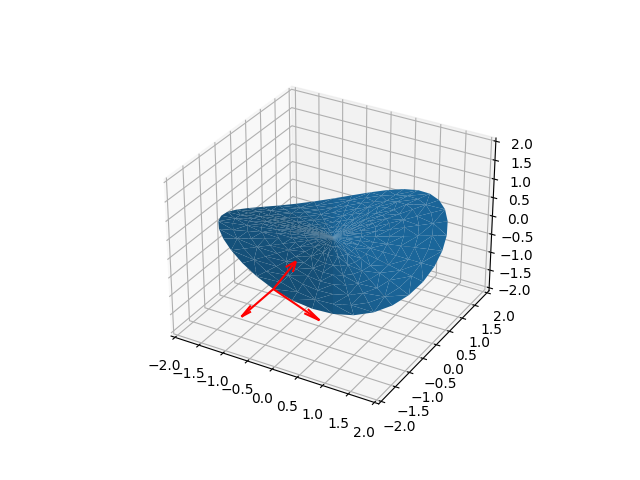
\includegraphics[width=0.7\columnwidth]{bsp_7.png}
\end{figure}

Zuerst suchen wir einen Normalvektor für jeden Punkt $(x,y,z)\in \Omega$:
\begin{align*}
	\bm{n} = \frac{\partial}{\partial r}\begin{pmatrix} 2r\cos(t)\\ 2r\sin(t)\\ r\cos(t)\sin(t) \end{pmatrix} \times \frac{\partial}{\partial t}\begin{pmatrix}
	2r\cos(t)\\ 2r\sin(t)\\ r\cos(t)\sin(t) \end{pmatrix} = \begin{pmatrix}
	-2r\sin^3(t)\\ -2r\cos^3(t)\\ 4r \end{pmatrix}
\end{align*}

Normieren ist nicht notwendig, da wir uns nur für die Orientierung interessieren. 

Nun zum Tangentialvektor auf $\partial\Omega = \{(2\cos(t), 2\sin(t), \cos(t)\sin(t))\in \mathbb{R}^3: 0 \leq t < 2\pi\}$:

\begin{align*}
	\tilde{\bm{t}} = \left(\frac{\partial}{\partial t} 2\cos(t), \frac{\partial}{\partial t} 2\sin(t), \frac{\partial}{\partial t} \cos(t)\sin(t)\right)^\top = (-2\sin(t), 2\cos(t), \cos^2(t)-\sin^2(t))^\top\\
	||\tilde{\bm{t}}|| = \sqrt{4\sin^2(t)+4\cos^2(t)+(\cos^2(t)-\sin^2(t))^2} = \sqrt{(\cos^2(t)-\sin^2(t))^2 + 4}\\
	\bm{t} := \frac{\tilde{\bm{t}}}{||\tilde{\bm{t}}||}
\end{align*}

\begin{align*}
	\bm{\nu} = \bm{n} \times \bm{\tilde{t}} = \begin{pmatrix} 8\cos(t)+2\cos^5(t)-2\sin^2(t)\cos^3(t)\\ -2\sin^3(t)\cos^2(t)+2\sin^5(t)+8\sin(t)\\ 4\sin(t)\cos^3(t)+4\sin^3(t)\cos(t) \end{pmatrix} = \begin{pmatrix} 8\cos(t)+2\cos^3(t)(\cos^2(t)-\sin^2(t))\\ 8\sin(t)+2\sin^3(t)(\sin^2(t)-\cos^2(t))\\ 4\sin(t)\cos(t)(\cos^2(t)+\sin^2(t)) \end{pmatrix}
\end{align*}

Die Bedingungen für den Stoke'schen Integralsatz im $\mathbb{R}^3$ sind:
\begin{itemize}
	\item $\Omega$ ist eine Teilmenge des $\mathbb{R}^3$
	\item $\Omega$ ist das Bild von $\phi \in C^2$ unter einer beschränkten Teilmenge des $\mathbb{R}^2$
\end{itemize}

Es gilt nun also
\begin{align*}
	\int_\Omega (rot \bm{F})^\top \cdot \bm{n} d\mathcal{H}^2 =	\int_{\partial\Omega} \bm{F}\cdot \bm{t} d\mathcal{H}^1 =\\
	\int_0^{2\pi} \frac{1}{\sqrt{(\cos^2(t)-\sin^2(t))^2 + 4}} (\cos(t)\sin(t), -\cos(t)\sin(t), 2\sin(t)) \cdot \begin{pmatrix} -2\sin(t)\\ 2\cos(t)\\ \cos^2(t)-\sin^2(t) \end{pmatrix} dt =\\
	\int_0^{2\pi} \frac{-2\sin^2(t)\cos(t) - 2\sin(t)\cos^2(t) + 2\sin(t)\cos^2(t) - 2\sin^3(t)}{\sqrt{(\cos^2(t)-\sin^2(t))^2 + 4}} dt = \int_0^{2\pi} \frac{-2\sin^2(t) (\sin(t)+\cos(t))}{\sqrt{(\cos^2(t)-\sin^2(t))^2 + 4}} dt
\end{align*}

Definieren wir $f(t)$ als das was im Integral steht so gilt $\forall t \in [0, \pi):$
\begin{align*}
	-f(t+\pi) = -\frac{-2\sin^2(t+\pi) (\sin(t+\pi)+\cos(t+\pi))}{\sqrt{(\cos^2(t+\pi)-\sin^2(t+\pi))^2 + 4}} =\\
	-\frac{-2\sin^2(t) (-\sin(t)-\cos(t))}{\sqrt{(\cos^2(t)-\sin^2(t))^2 + 4}} =
	\frac{-2\sin^2(t) (\sin(t)+\cos(t))}{\sqrt{(\cos^2(t)-\sin^2(t))^2 + 4}} = f(t)
\end{align*}

Woraus folgt
\begin{align*}
	\int_\Omega (rot \bm{F})^\top \cdot \bm{n} d\mathcal{H}^2 = \int_0^{2\pi} f(t) dt = \int_0^{\pi} f(t) dt + \int_\pi^{2\pi} f(t) dt = \int_0^{\pi} f(t) dt + \int_0^{\pi} f(t+\pi) dt = 0
\end{align*}

\newpage

\subsection*{Beispiel 8}
\begin{angabe*}
	Sei $\bm{F}(x,y,z):=(x^2y, z^2, x+y+z^3)^\top$. Betrachte
	\begin{align*}
		\Omega := \{(x,y,z) \in \mathbb{R}^3: z=(\sqrt{x^2+y^2}+1)(\sqrt{x^2+y^2}-1)(x^2+y^2), x^2+y^2 < 1\}.
	\end{align*}
	Setzte $\bm{n}$ das normierte Normalvektorfeld auf $\Omega$ mit positiver $z$-Koordinate. Berechen Sie
	\begin{align*}
		\int_\Omega (rot \bm{F})^\top \cdot \bm{n} d\mathcal{H}^2.
	\end{align*}
\end{angabe*}

\begin{figure}[h!]
	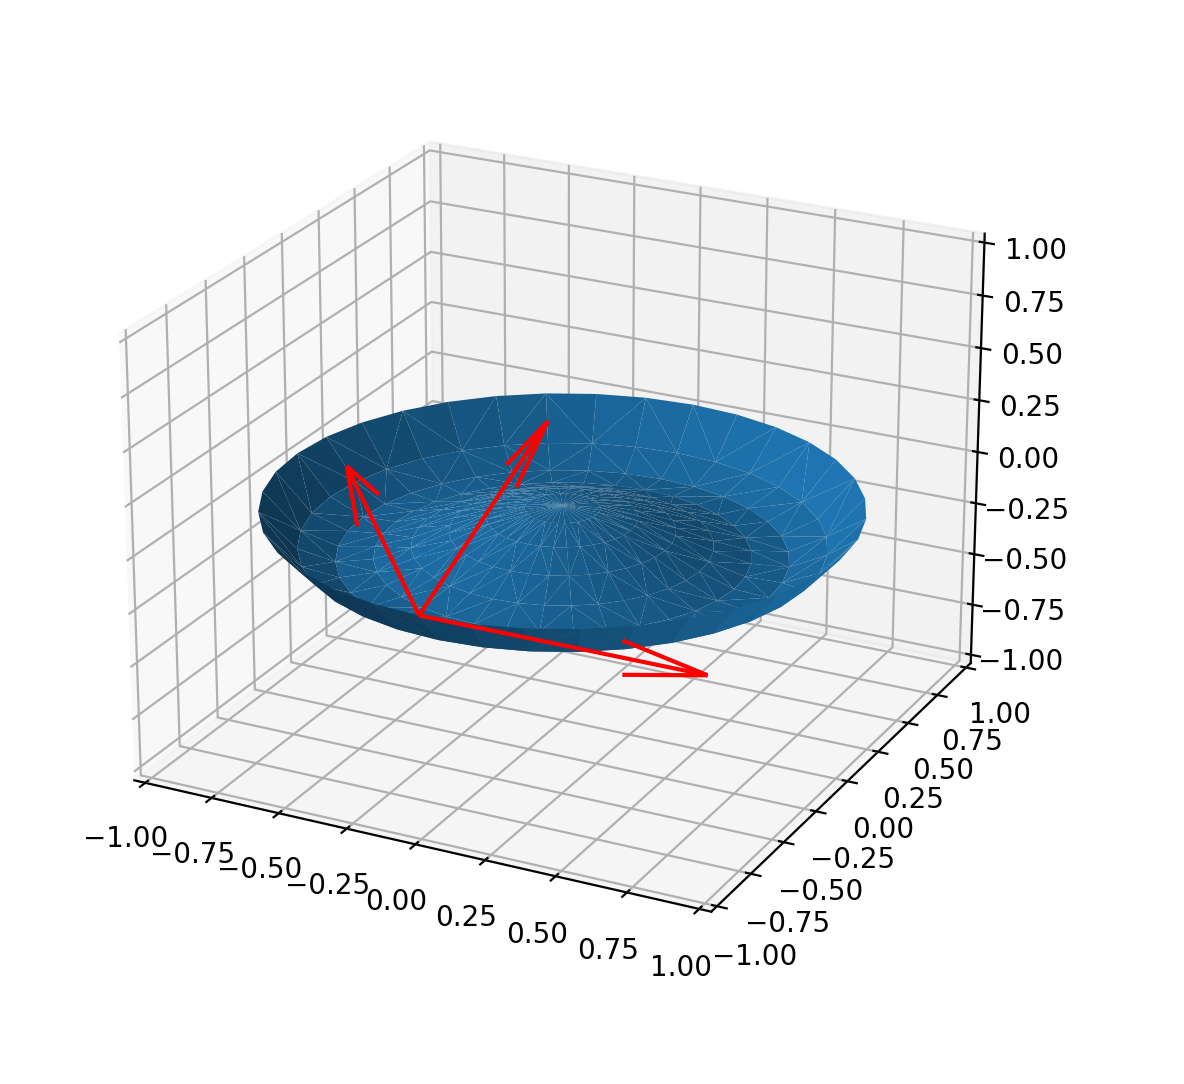
\includegraphics[width=0.5\columnwidth]{bsp_8.png}
\end{figure}

Wir suchen zuerst die Normalvektoren auf $\Omega$ mit positiver $z$-Koordinate. Für jeden Punkt $(x,y,z(x,y)) \in \Omega$ ist $\bm{n}$ ein normierter Normalvektor:
\begin{align*}
	\tilde{\bm{n}} := \left(-\frac{\partial}{\partial x} z(x,y), -\frac{\partial}{\partial y} z(x,y), 1\right)^\top = (-2x(2x^2+2y^2-1), -2y(2x^2+2y^2-1), 1)^\top\\
	||\tilde{\bm{n}}|| = \sqrt{4x^2(2x^2+2y^2-1)^2 + 4y^2(2x^2+2y^2-1)^2 + 1} = \sqrt{(4x^2+4y^2)(2x^2+2y^2-1)^2+1}\\
	\bm{n}:= \frac{\tilde{\bm{n}}}{||\tilde{\bm{n}}||}
\end{align*}

Um den Integralsatz von Stokes in $\mathbb{R}^3$ anwenden zu können müssen wir nun einen Tangentialvektor $\bm{t}$ für jeden Punkt in $\partial\Omega$ finden.
\begin{align*}
	\partial\Omega = \{(x,y,(\sqrt{x^2+y^2}+1)(\sqrt{x^2+y^2}-1)(x^2+y^2)) \in \mathbb{R}^3: x^2+y^2=1\} = \{(x,y,0) \in \mathbb{R}^3: x^2+y^2=1\}
\end{align*}
\begin{align*}
	\bm{t} = (-y, x, 0)^\top && ||\bm{t}|| = \sqrt{y^2+x^2} = 1\\
\end{align*}

Auf $\partial\Omega$ gilt $\tilde{\bm{n}}=(-2x(2-1), -2y(2-1), 1)^\top = (-2x, -2y, 1)^\top$.
\begin{align*}
	\bm{\nu} = \tilde{\bm{n}} \times \bm{t} = \begin{pmatrix} x\\ y\\ 2x^2+2y^2 \end{pmatrix} = \begin{pmatrix} x\\ y\\ 2 \end{pmatrix}\\
	\det(\bm{\nu}, \bm{t}, \bm{n}) = \det\begin{pmatrix}
		x & -y & -2x\\
		y & x  & -2y\\
		2 & 0  & 1
	\end{pmatrix} = x^2+4y^2+4x^2+y^2 = 5(x^2+y^2) = 5 > 0
\end{align*}

Überprüfen wir als nächstes die Bedingungen des Integralsatzes von Stokes in $\mathbb{R}^3$:

\begin{itemize}
	\item $\Omega \subseteq \mathbb{R}^3$
	\item $\Omega$ ist das Bild einer $C^2$-Abbildung:
	\begin{align*}
		D := \{(x,y)\in\mathbb{R}^2: x^2+y^2 < 1\}\\
		\phi: D \rightarrow \mathbb{R}^3, \phi(x, y) := (x, y, (\sqrt{x^2+y^2}+1)(\sqrt{x^2+y^2}-1)(x^2+y^2))
	\end{align*}
	Es gilt $\phi(D)=\Omega$ und $\phi \in C^2(\bar{D})$.
	\item $D$ ist beschränkt.
\end{itemize}

Also gilt
\begin{align*}
	\int_\Omega (rot\bm{F})^\top \cdot \bm{n} d\mathcal{H}^2 = \int_{\partial\Omega} \bm{F}^\top \cdot \bm{t} d\mathcal{H}^1 = \int_{\partial\Omega} (x^2y, 0, x+y) \cdot \begin{pmatrix} -y\\ x\\ 0 \end{pmatrix} d\mathcal{H}^1 =\\
	\int_{\partial\Omega} -x^2y^2 d\mathcal{H}^1 = -\int_{0}^{2\pi} \cos^2(\theta) \sin^2(\theta) d\theta = -\frac{\pi}{4}
\end{align*}

Wobei die vorletzte Gleichung aus der Transformationsformel für $D=[0,2\pi)$ und $\phi(\theta)=(\cos(\theta), \sin(\theta), 0)$ folgt.

\end{document}
